\SetPicSubDir{ch-methodology}
\SetExpSubDir{ch-methodology}

\chapter{Methodology}
\label{methodology}

\section{Solvers}
We will employ five QUBO-solving-methods:
\begin{enumerate}
    \item Quantum Annealing
    \item Neural Network Quantum States
    \item Quantum Approximate Optimization Algorithm
    \item GUROBI Optimizer
    \item Fixstars Amplify QUBO Solver
\end{enumerate}
The following sections will provide more information on the solvers used for each method.

\subsection{Quantum Annealing}
We will use quantum annealers from D-wave Systems as the solver for Quantum Annealing. D-Wave Systems, a Canadian-based company, currently produces the most popular commercially available quantum annealing hardware and uses superconducting qubits to represent binary variables in their annealers \cite{b14}.  Given a target QUBO problem to solve, the process for using a D-Wave Systems Quantum Processing Unit (QPU) is as follows:

\begin{enumerate}
    \item \textbf{Problem Definition} QUBO problem is first converted to its corresponding Ising model Hamiltonian on the local device.
    \item \textbf{Minor Embedding} As the Quantum Processing Unit (QPU) used by D-Wave is not fully connected as shown in \autoref{pegasustopology}, a single variable in the Ising model may need to be represented by multiple qubits called a \textit{chain} which are forced to return the same value with large interaction terms \cite{b16}.
    \item \textbf{Programming} The parameters of the annealing process are set, which consists of the bias for each qubit (represents magnetic field acting on each qubit) and coupler strength (represents variable interaction).
    \item \textbf{Initialization} The QPU is initialized in the ground state of an easy-to-implement initial Hamiltonian. The qubits are prepared to be in a superposition of all possible states.
    \item \textbf{Annealing} The system evolves with a time-varying Hamiltonian.
    \item \textbf{Readout of solution} The spin values of the qubits are measured and stored as a possible solution.
    \item \textbf{Resample} As the finite-time quantum annealing process does not guarantee that the system ends up in the ground state, we repeat the sampling to obtain many possible solutions that are likely to be the ground state of the initial Hamiltonian.
\end{enumerate}

\begin{figure}[h!]
    \centering
    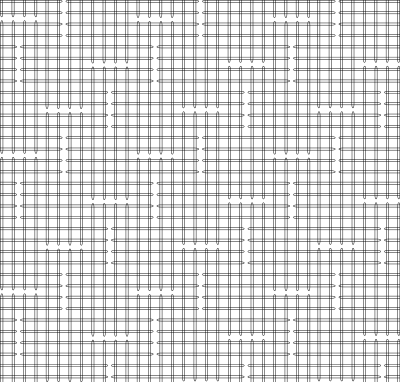
\includegraphics[width=0.6\linewidth]{images/pegasus_topology.png}
    \caption{A view of the D-Wave pegasus topology where each line represents a qubit and intersections represent available couplers~\protect\cite{dwaveadvantage}}
    \label{pegasustopology}
\end{figure}

The experiments will be conducted with the Advantage 4.1 solver, which has a Pegasus graph topology with up to 5640 qubits and 40484 couplers \cite{dwaveadvantage}. The Pegasus topology allows for 15 couplers per qubit which are arranged as shown in \autoref{pegasustopology}.


\subsection{Neural-Network Quantum States}
For Neural-Network Quantum States, we will use a Python library MAPALUS that is implemented in Python. We will use both RBM (with $2n$ hidden nodes) and MLP (with one positive real output, $1$ hidden layers of size $2n$, and the ReLU activation function) as the underlying architecture. The NNQS will be used to simulate a quantum annealing process with a time-dependent Hamiltonian that follows \autoref{eqn:annealinghamiltonian}. 

Three training algorithms will be employed---Direct, Stepwise Annealing, and Continuous Annealing. In direct training, the normalized anneal fraction $s$ is held constant at $1$ for all epochs. In Stepwise Annealing, the normalized anneal fraction $s$ starts at $0$ and will be incremented by $0.1$ each time while the NNQS is trained until convergence or the $100$ epoch limit. In Continuous Annealing, we first set an epoch limit of $1100$ and for each epoch $i$, use $s = \frac{i}{1100}$ as the anneal fraction to train the NNQS for a single epoch. The learning rate is $0.001$ and the optimizer is RMSprop.

\subsection{Quantum Approximate Optimization Algorithm}
We will employ the implementation of QAOA in Qiskit with different values of $p$ using a backend hosted on the IBM Quantum Platform, which provides limited access to quantum computers with up to 127 qubits \cite{b24}.

\subsection{GUROBI Optimizer}
The GUROBI optimizer is used as a classical solver as a state-of-the-art commercial solver. GUROBI is a state-of-the-art commercial solver, which is free for academic use \cite{b26}.

\subsection{Fixstars Amplify QUBO Solver}
The Fixstar Amplify QUBO solver API is provided for free as well \cite{b12}.

\section{Benchmark datasets}
We use 3 randomly generated problem sets to benchmark our QUBO solvers. These problems were chosen as they are commonly used to represent NP-hard problems to measure the performance of QUBO solvers and are relatively easy to encode into QUBO form with a linear number of variables. They are the not-all-equal 3-satisfiability (NAE3SAT), max-cut, and the Sherrington-Kirkpatrick (SK) model.

\subsection*{Not-all-equal 3-satisfiability (NAE3SAT)}
The NAE3SAT problem is a variant of the boolean satisfiability problem where each problem instance consists of $n$ boolean variables $(x_1, x_2, ..., x_n)$ and $m$ clauses that each combine three variables or negations of the variables. The objective is to find an assignment of boolean values to the variables such that the three values in each clause are not all the same. The ratio of clauses to variables $\rho = \frac{m}{n}$ determines whether such an assignment exists.

For example, for the clause $(x_2, x_4, \neg x_5)$, a valid assignment must have at least one of $x_2, x_4, \neg x_5$ as true and at least one as false.


\subsection*{Max-cut}
\subsection*{Sherrington-Kirkpatrick (SK) model}
Parisi [6] provides a formula (for proof, see [7])
that, when numerically evaluated [8, 9, 1], shows for typical instances,
\begin{equation*}
    \lim_{n\rightarrow \infty} \argmin \frac{E}{n} = -0.763166...
\end{equation*}
(get from this paper https://quantum-journal.org/papers/q-2022-07-07-759/pdf/)

Each problem set is generated for 6 different sizes, $(10, 25, 50, 75, 100, 250)$, with 10 different random seeds $(0-9)$.



%We plan to use a subset of the 3296 QUBO problems provided by MQLib as our benchmark dataset. These problems are publicly accessible and contain both "real-world problem instances" and randomly generated problems \cite{b12}. The dataset also contains problems of various sizes and densities. The exact benchmark dataset will be determined after further testing to determine the input limits of each solver. Each QUBO problem will first be converted into an Ising model problem and then passed to each of the solvers.

\section{Performance evaluation}
For each solver, we will have two performance metrics 
\begin{enumerate}
    \item The probability of finding the optimal solution
    \item The average normalized performance, used in \cite{b34}, which is 
    \begin{equation}
        r = \frac{1}{n} \sum_n \frac{E_{\text{sol}} - E_{\min}}{E_{\max} - E_{\min}}
    \end{equation}
\end{enumerate}

The normalized performance has the range of possible energies in the denominator to account for both negative and positive ground-state energies. 